\documentclass[12pt,a4paper]{article}

% =====================================================
% PACOTES
% =====================================================
\usepackage[utf8]{inputenc}
\usepackage[T1]{fontenc}
\usepackage[brazil]{babel}
\shorthandoff{"}
\usepackage{geometry}
\usepackage{graphicx}
\usepackage{fancyhdr}
\usepackage{titlesec}
\usepackage[table]{xcolor}
\usepackage{hyperref}
\usepackage{setspace}
\usepackage{enumitem}
\usepackage{newtxtext,newtxmath}
\usepackage[most]{tcolorbox}
\usepackage{float}
\usepackage{tikz}
\usetikzlibrary{arrows.meta, positioning, babel}
\usepackage{tabularx}

\geometry{
    top=2.5cm,
    bottom=3cm,
    left=1.5cm,
    right=1.5cm
}

\onehalfspacing

% =====================================================
% CORES PERSONALIZADAS
% =====================================================
\definecolor{azulTitulo}{RGB}{30,60,90}
\definecolor{azulObjetivos}{RGB}{30,60,90}
\definecolor{cinzaCodigo}{RGB}{245,245,245}
\definecolor{vermelhoCodigo}{RGB}{180,50,50}
\definecolor{mostarda}{RGB}{204,153,0}

% =====================================================
% BOXES
% =====================================================
\newtcolorbox{boxAtividade}[1][]{
    breakable,
    enhanced,
    colback=azulTitulo!5,
    colframe=azulTitulo,
    boxrule=0pt,
    arc=6pt,
    outer arc=6pt,
    boxsep=0pt,
    left=14pt,
    right=14pt,
    top=16pt,
    bottom=14pt,
    title=#1,
    coltitle=white,
    colbacktitle=azulTitulo,
    fonttitle=\bfseries,
    attach boxed title to top left={
        yshift=-3mm,
        xshift=6mm
    },
    boxed title style={
        sharp corners,
        boxrule=0pt
    }
}

\newtcolorbox{boxCodigo}{
    breakable,
    colback=cinzaCodigo,
    colframe=vermelhoCodigo,
    boxrule=0.8pt,
    arc=2pt,
    left=6pt,
    right=6pt,
    top=6pt,
    bottom=6pt,
    borderline={0.5pt}{0pt}{vermelhoCodigo,dashed}
}

\definecolor{verdeResultado}{RGB}{22,101,52}
\newtcolorbox{boxResultado}[1][]{
    breakable,
    enhanced,
    colback=verdeResultado!6,
    colframe=verdeResultado,
    boxrule=0pt,
    arc=6pt,
    outer arc=6pt,
    boxsep=0pt,
    left=14pt,
    right=14pt,
    top=16pt,
    bottom=14pt,
    title=#1,
    coltitle=white,
    colbacktitle=verdeResultado,
    fonttitle=\bfseries,
    attach boxed title to top left={
        yshift=-3mm,
        xshift=6mm
    },
    boxed title style={
        sharp corners,
        boxrule=0pt
    }
}

% =====================================================
% CABEÇALHO E RODAPÉ
% =====================================================
\pagestyle{fancy}
\fancyhf{}
\fancyhead[L]{
    % Tenta carregar a logo se o caminho estiver correto, senão ignora
    \IfFileExists{../../uc-topicos-avancados-latex/figures/garopaba_horizontal_marca2015_PNG.png}{
        \includegraphics[height=1.4cm]{../../uc-topicos-avancados-latex/figures/garopaba_horizontal_marca2015_PNG.png}
    }{IFSC - Garopaba}
}
\fancyhead[R]{
    \textbf{Roteiro Prático 07}\\
    UC – Tópicos Avançados em Informática\\
    Técnico Integrado em Informática
}
\fancyfoot[L]{\small\textit{Integração Frontend com API - Roteiro 07}}
\fancyfoot[R]{\small Página \thepage}
\renewcommand{\footrulewidth}{2.4pt}
\setlength{\headheight}{45pt}

% =====================================================
% ESTILO DE SEÇÃO
% =====================================================
\titleformat{\section}
{\normalfont\Large\bfseries\color{azulTitulo}}
{\thesection}
{1em}
{}
[\vspace{0.3cm}\hrule]

\begin{document}

\section*{Roteiro Prático 07 — Integração Frontend com API no Flask}

\begin{boxAtividade}[Objetivos da Aula]
Ao final desta aula, o estudante será capaz de:
\begin{itemize}
    \item Compreender o conceito de \textbf{desacoplamento} (separação de Frontend e Backend);
    \item Transformar uma aplicação Flask em uma \textbf{API REST} que responde \textbf{JSON};
    \item Consumir rotas de API utilizando a \textbf{Fetch API} do JavaScript no navegador;
    \item Manipular a árvore \textbf{DOM} para exibir, cadastrar e remover elementos sem recarregar a página.
\end{itemize}
\end{boxAtividade}

\subsection*{Ferramentas Necessárias}

Python, Flask, JavaScript básico, HTML5 semântico, navegador web, Git.

\subsection*{De onde viemos (Roteiro 05) para onde vamos (Roteiro 07)}

Para compreender o salto tecnológico de hoje, vamos analisar as diferenças fundamentais entre o modelo de desenvolvimento dinâmico clássico (\textbf{Roteiro 05}) e a arquitetura moderna baseada em APIs (\textbf{Roteiro 07}):

\vspace{0.3cm}
\begin{center}
\small
\renewcommand{\arraystretch}{1.4}
\rowcolors{2}{azulTitulo!5}{white}
\begin{tabularx}{\linewidth}{|p{3.2cm}|X|X|}
\hline
\rowcolor{azulTitulo}
\color{white}\textbf{Aspecto} & 
\color{white}\textbf{Roteiro 05: Flask CRUD (SSR)} & 
\color{white}\textbf{Roteiro 07: API e Fetch (CSR)} \\ \hline

\textbf{Papel do Flask} & 
\textbf{Injeção de Layout + Dados:} O Flask processa os dados e monta o HTML no servidor usando Jinja2. & 
\textbf{Servidor de Dados Puro:} O Flask vira uma API REST que apenas recebe e responde JSON. \\ \hline

\textbf{Navegação} & 
\textbf{Recarregamento Completo:} Toda ação do usuário (cadastrar/deletar) recarrega a página inteira (tela pisca). & 
\textbf{Atualização Cirúrgica:} O JavaScript intercepta ações e atualiza cirurgicamente apenas os nós alterados. \\ \hline

\textbf{Tráfego de Dados} & 
\textbf{Form Data:} Dados via formulário físico do HTML (\texttt{request.form}). & 
\textbf{JSON:} Dados padronizados e estruturados no corpo da requisição (\texttt{request.get\_json()}). \\ \hline

\textbf{Reuso de Código} & 
\textbf{Preso ao Layout:} Backend acoplado ao HTML/Jinja2. Impossível reutilizar para um app celular. & 
\textbf{Totalmente Desacoplado:} O mesmo backend atende o site web, apps móveis (iOS/Android) ou outros servidores. \\ \hline
\end{tabularx}
\end{center}

\newpage

\subsection*{Comparação Prática de Fluxo e Código}

\textbf{1. Rota de Cadastro no Flask}
\begin{boxCodigo}
\begin{verbatim}
# ROTEIRO 05 (Jinja2 / Form Data)
@app.route("/alunos", methods=["POST"])
def adicionar_aluno():
    nome = request.form["nome"]
    idade = int(request.form["idade"])
    alunos.append(Aluno(nome, idade))
    return redirect("/")  # Recarrega a tela

# ROTEIRO 07 (API REST / JSON)
@app.route("/api/alunos", methods=["POST"])
def api_adicionar_aluno():
    dados = request.get_json()
    novo_aluno = Aluno(dados["nome"], int(dados["idade"]))
    alunos.append(novo_aluno)
    return jsonify(novo_aluno.to_dict()), 201  # Retorna dados puros
\end{verbatim}
\end{boxCodigo}

\textbf{2. Exibição de Dados no Frontend}
\begin{boxCodigo}
\begin{verbatim}
<!-- ROTEIRO 05 (Jinja2 no Servidor) -->
<ul>
    {% for aluno in alunos %}
        <li>{{ aluno.nome }} - {{ aluno.idade }} anos</li>
    {% endfor %}
</ul>

<!-- ROTEIRO 07 (DOM Dinâmico no Cliente com JS) -->
<ul id="lista-alunos"></ul>
<script>
    fetch('/api/alunos')
        .then(res => res.json())
        .then(alunos => {
            alunos.forEach(aluno => {
                const li = document.createElement('li');
                li.innerHTML = `<strong>${aluno.nome}</strong> - ${aluno.idade} anos`;
                listaAlunos.appendChild(li);
            });
        });
</script>
\end{verbatim}
\end{boxCodigo}

\newpage

\subsection*{Esboço (Croqui) da Interface}

Abaixo está o croqui representando como a interface Single Page Application (SPA) será estruturada visualmente. Os dados serão carregados, inseridos e removidos dinamicamente da lista sem recarregar a tela:

\begin{center}
\begin{tikzpicture}[
    scale=0.95,
    every node/.style={font=\small},
    browser/.style={draw=black!70, thick, fill=white, minimum width=12cm, minimum height=8.5cm, rounded corners=3pt},
    formbox/.style={draw=blue!60!black, thick, fill=blue!5, minimum width=11cm, minimum height=3cm, rounded corners=4pt},
    inputbox/.style={draw=black!40, fill=white, minimum width=8.5cm, minimum height=0.6cm, align=left},
    button/.style={draw=azulTitulo, fill=azulTitulo, text=white, font=\bfseries\small, minimum width=3.5cm, minimum height=0.7cm, rounded corners=2pt},
    btnremover/.style={draw=vermelhoCodigo, fill=vermelhoCodigo, text=white, font=\bfseries\tiny, minimum width=1.5cm, minimum height=0.5cm, rounded corners=1pt},
    listitem/.style={draw=black!20, fill=gray!2, minimum width=11cm, minimum height=0.8cm, rounded corners=2pt}
]

    % Janela do Navegador
    \node[browser] (win) at (6, -4.25) {};
    
    % Barra de Título / URL
    \draw[fill=gray!20, draw=black!40] (0, 0) rectangle (12, 0.5);
    \draw[fill=white, draw=black!30] (1.5, 0.1) rectangle (11.5, 0.4);
    \node[anchor=west, font=\tiny\ttfamily] at (1.6, 0.25) {http://localhost:5000/};
    \draw[fill=red!70] (0.3, 0.25) circle (0.08);
    \draw[fill=yellow!70] (0.6, 0.25) circle (0.08);
    \draw[fill=green!70] (0.9, 0.25) circle (0.08);

    % Título da Página
    \node[anchor=west, font=\large\bfseries\color{azulTitulo}] at (0.5, -0.6) {Controle de Alunos (Modo API)};

    % Formulário de Cadastro (Caixa)
    \node[formbox, anchor=north west] (form) at (0.5, -1.2) {};
    \node[anchor=west, font=\bfseries\color{blue!80!black}] at (0.7, -1.5) {Formulário de Cadastro (id="formulario-cadastro")};
    
    % Campos do formulário
    \node[inputbox, anchor=west] (input1) at (2.8, -2.1) {\,\,Digite o nome completo};
    \node[anchor=east, font=\bfseries, align=right] at (2.7, -2.1) {Nome do\\Aluno:};
    
    \node[inputbox, anchor=west] (input2) at (2.8, -2.9) {\,\,Ex: 17};
    \node[anchor=east, font=\bfseries] at (2.7, -2.9) {Idade:};
    
    % Botão Cadastrar
    \node[button, anchor=west] (btnsub) at (2.8, -3.7) {Cadastrar via API};

    % Separador (hr)
    \draw[thick, black!30, dashed] (0.5, -4.4) -- (11.5, -4.4);

    % Lista de Alunos (Título)
    \node[anchor=west, font=\large\bfseries\color{azulTitulo}] at (0.5, -4.8) {Alunos Cadastrados};

    % Itens da Lista (ul / li)
    \node[listitem, anchor=north west] (li1) at (0.5, -5.2) {};
    \node[anchor=west] at (0.7, -5.6) {\textbf{João Silva} - 17 anos (Média: 8.5)};
    \node[btnremover, anchor=east] at (11.3, -5.6) {Remover};

    \node[listitem, anchor=north west] (li2) at (0.5, -6.2) {};
    \node[anchor=west] at (0.7, -6.6) {\textbf{Maria Souza} - 16 anos (Média: 9.0)};
    \node[btnremover, anchor=east] at (11.3, -6.6) {Remover};

\end{tikzpicture}
\end{center}

\subsection*{Fluxo Geral de Comunicação (REST / SPA)}

Abaixo está representado o fluxo de comunicação em segundo plano (assíncrono) entre o cliente (navegador/JavaScript) e o servidor de API (Flask):

\begin{center}
\begin{tikzpicture}[
    node distance=1.5cm and 2.5cm,
    box/.style={draw=azulTitulo, fill=azulTitulo!5, thick, rounded corners=4pt, minimum width=3.5cm, minimum height=1cm, align=center, font=\small},
    db/.style={draw=mostarda, fill=mostarda!5, thick, rounded corners=4pt, minimum width=3.5cm, minimum height=1cm, align=center, font=\small},
    arrow/.style={thick, -{Stealth[scale=1.2]}, draw=azulTitulo},
    apiarrow/.style={thick, dashed, -{Stealth[scale=1.2]}, draw=vermelhoCodigo}
]
    % Elementos
    \node[box] (front) at (0, 0) {Navegador / Frontend\\(HTML + JS Fetch)};
    \node[box] (back) at (7.5, 0) {Servidor Flask\\(app.py / API REST)};
    \node[db] (db) at (7.5, -2.5) {Memória RAM\\(Lista Python)};

    % Setas e Fluxos
    \draw[arrow] ([yshift=0.3cm]front.east) -- node[above, font=\tiny\sffamily] {1. GET /api/alunos} ([yshift=0.3cm]back.west);
    \draw[apiarrow] ([yshift=0.0cm]back.west) -- node[below, font=\tiny\sffamily] {2. JSON: [Alunos]} ([yshift=0.0cm]front.east);

    \draw[arrow] ([yshift=-0.4cm]front.east) -- node[above, font=\tiny\sffamily] {3. POST /api/alunos (JSON)} ([yshift=-0.4cm]back.west);
    \draw[apiarrow] ([yshift=-0.7cm]back.west) -- node[below, font=\tiny\sffamily] {4. JSON: Novo Aluno (201)} ([yshift=-0.7cm]front.east);

    % Conexão interna
    \draw[arrow] ([xshift=-0.5cm]back.south) -- node[left, font=\tiny\sffamily] {Gravar / Deletar} ([xshift=-0.5cm]db.north);
    \draw[apiarrow] ([xshift=0.5cm]db.north) -- node[right, font=\tiny\sffamily] {Ler dados} ([xshift=0.5cm]back.south);
\end{tikzpicture}
\end{center}

\newpage

\subsection*{Roteiro Prático}

\begin{boxAtividade}[Parte 0 – Preparando o Ambiente do Zero]
\begin{center}
\begin{tikzpicture}[
    stepbox/.style={draw=azulTitulo, fill=azulTitulo!5, thick, rounded corners=3pt, minimum width=2.6cm, minimum height=0.9cm, align=center, font=\scriptsize},
    arrow/.style={thick, -{Stealth[scale=1.0]}, draw=azulTitulo}
]
    \node[stepbox] (s1) at (0, 0) {1. Criar Pasta\\do Projeto};
    \node[stepbox] (s2) at (3.4, 0) {2. Criar e Ativar\\venv};
    \node[stepbox] (s3) at (6.8, 0) {3. Instalar\\Flask (pip)};
    \node[stepbox] (s4) at (10.2, 0) {4. Criar Pasta\\\texttt{templates/}};

    \draw[arrow] (s1) -- (s2);
    \draw[arrow] (s2) -- (s3);
    \draw[arrow] (s3) -- (s4);
\end{tikzpicture}
\end{center}

\vspace{0.2cm}

Para garantir que o projeto seja construído do absoluto zero (sem dependências obrigatórias de aulas anteriores), abra o terminal do seu computador e execute os comandos abaixo para criar a pasta, configurar o ambiente virtual isolado e instalar o Flask:

\begin{boxCodigo}
\begin{verbatim}
# 1. Crie a pasta do projeto e entre nela
mkdir roteiro07-integracao-api
cd roteiro07-integracao-api

# 2. Crie e ative o ambiente virtual (venv)
# No macOS/Linux:
python3 -m venv venv
source venv/bin/activate

# No Windows (CMD):
python -m venv venv
venv\Scripts\activate

# 3. Instale o Flask e suas dependências
pip install Flask

# 4. Crie a subpasta para as telas HTML
mkdir templates
\end{verbatim}
\end{boxCodigo}
\end{boxAtividade}

\newpage

\begin{boxAtividade}[Parte 1 – Criando o Modelo (classe Aluno)]
\begin{center}
\begin{tikzpicture}[
    stepbox/.style={draw=azulTitulo, fill=azulTitulo!5, thick, rounded corners=3pt, minimum width=2.6cm, minimum height=0.9cm, align=center, font=\scriptsize},
    arrow/.style={thick, -{Stealth[scale=1.0]}, draw=azulTitulo}
]
    \node[stepbox] (s1) at (0, 0) {1. Instanciar\\Objeto \texttt{Aluno}};
    \node[stepbox] (s2) at (3.4, 0) {2. Gerar ID Único\\e Incrementar};
    \node[stepbox] (s3) at (6.8, 0) {3. Adicionar Notas\\e Calcular Média};
    \node[stepbox] (s4) at (10.2, 0) {4. Serializar via\\\texttt{to\_dict()} (JSON)};

    \draw[arrow] (s1) -- (s2);
    \draw[arrow] (s2) -- (s3);
    \draw[arrow] (s3) -- (s4);
\end{tikzpicture}
\end{center}

\vspace{0.2cm}

Para podermos deletar ou editar alunos específicos através de chamadas de API, precisamos que a classe \texttt{Aluno} possua um ID único incremental e consiga exportar seus dados como um dicionário Python (o qual o Flask pode converter em texto bruto JSON).

Crie o arquivo \texttt{aluno.py} com a seguinte estrutura completa:

\begin{boxCodigo}
\begin{verbatim}
class Aluno:
    contador = 1  # Contador estático para gerar IDs únicos

    def __init__(self, nome, idade):
        self.id = Aluno.contador
        self.nome = nome
        self.idade = idade
        self.notas = []
        Aluno.contador += 1

    def adicionar_nota(self, nota):
        self.notas.append(nota)

    def calcular_media(self):
        if not self.notas:
            return 0
        return sum(self.notas) / len(self.notas)

    def aprovado(self):
        return self.calcular_media() >= 7

    # Transforma o objeto em um dicionário compatível com JSON
    def to_dict(self):
        return {
            "id": self.id,
            "nome": self.nome,
            "idade": self.idade,
            "media": self.calcular_media(),
            "aprovado": self.aprovado(),
        }
\end{verbatim}
\end{boxCodigo}
\end{boxAtividade}

\newpage

\begin{boxAtividade}[Parte 2 – Construindo a API no Backend (app.py)]
\begin{center}
\begin{tikzpicture}[
    stepbox/.style={draw=azulTitulo, fill=azulTitulo!5, thick, rounded corners=3pt, minimum width=2.6cm, minimum height=0.9cm, align=center, font=\scriptsize},
    arrow/.style={thick, -{Stealth[scale=1.0]}, draw=azulTitulo}
]
    \node[stepbox] (s1) at (0, 0) {\textbf{GET /}\\Retorna HTML};
    \node[stepbox] (s2) at (3.4, 0) {\textbf{GET /api/alunos}\\Retorna JSON};
    \node[stepbox] (s3) at (6.8, 0) {\textbf{POST /api/alunos}\\Cria Aluno + 201};
    \node[stepbox] (s4) at (10.2, 0) {\textbf{DELETE /api/...}\\Remove Aluno + 200};

    \draw[arrow] (s1) -- (s2);
    \draw[arrow] (s2) -- (s3);
    \draw[arrow] (s3) -- (s4);
\end{tikzpicture}
\end{center}

\vspace{0.2cm}

No arquivo \texttt{app.py}, faremos modificações importantes. A nossa rota principal \texttt{/} apenas entregará a página HTML base uma única vez. Todas as outras interações de dados (listar, cadastrar, deletar) serão feitas por rotas exclusivas de API prefixadas com \texttt{/api/}.

Crie ou substitua o conteúdo do arquivo \texttt{app.py} com a seguinte estrutura completa:
\end{boxAtividade}

\begin{boxCodigo}
\begin{verbatim}
from flask import Flask, jsonify, request, render_template
from aluno import Aluno

app = Flask(__name__)

# Banco de dados simulado em memória
alunos = []

# Inicializando com alguns dados de teste
aluno1 = Aluno("João Silva", 17)
aluno1.adicionar_nota(8.5)
aluno2 = Aluno("Maria Souza", 16)
aluno2.adicionar_nota(9.0)

alunos.append(aluno1)
alunos.append(aluno2)

# ==========================================
# 1. ROTA DE TELA (HTML Estático)
# ==========================================
@app.route("/", methods=["GET"])
def pagina_inicial():
    # Retorna o arquivo HTML sem injetar dados via Jinja2
    return render_template("index.html")

# ==========================================
# 2. ROTAS DE API (Endpoints JSON)
# ==========================================

# ROTA A: Listar Alunos (GET)
@app.route("/api/alunos", methods=["GET"])
def listar_alunos():
    # Converte Alunos para dicionários usando to_dict()
    alunos_dict = [aluno.to_dict() for aluno in alunos]
    return jsonify(alunos_dict), 200

# ROTA B: Adicionar um novo aluno (POST)
@app.route("/api/alunos", methods=["POST"])
def adicionar_aluno():
    # Extrai os dados do corpo da requisição JSON
    dados = request.get_json()
    nome = dados.get("nome")
    idade = dados.get("idade")

    # Valida os dados recebidos
    if not nome or not isinstance(idade, int):
        return jsonify({
            "error": "Dados inválidos. 'nome' deve ser string e 'idade' int."
        }), 400

    # Cria um novo objeto Aluno e adiciona à lista de alunos
    novo_aluno = Aluno(nome, idade)
    alunos.append(novo_aluno)

    return jsonify(novo_aluno.to_dict()), 201

# ROTA C: Remover Aluno (DELETE)
@app.route("/api/alunos/<int:id>", methods=["DELETE"])
def api_remover_aluno(id):
    global alunos
    aluno_existe = any(aluno.id == id for aluno in alunos)
    if not aluno_existe:
        return jsonify({"erro": "Aluno não encontrado"}), 404
    alunos = [aluno for aluno in alunos if aluno.id != id]
    return jsonify({"mensagem": "Aluno removido com sucesso"}), 200
\end{verbatim}
\end{boxCodigo}

\newpage

\begin{boxAtividade}[Parte 3 – Criando a Interface no Frontend (index.html)]
\begin{center}
\begin{tikzpicture}[
    stepbox/.style={draw=azulTitulo, fill=azulTitulo!5, thick, rounded corners=3pt, minimum width=2.6cm, minimum height=0.9cm, align=center, font=\scriptsize},
    arrow/.style={thick, -{Stealth[scale=1.0]}, draw=azulTitulo}
]
    \node[stepbox] (s1) at (0, 0) {\textbf{Carregar (GET)}\\Fetch + Injetar DOM};
    \node[stepbox] (s2) at (3.4, 0) {\textbf{Cadastrar (POST)}\\Fetch + Injetar DOM};
    \node[stepbox] (s3) at (6.8, 0) {\textbf{Remover (DELETE)}\\Fetch + Remover DOM};
    \node[stepbox] (s4) at (10.2, 0) {\textbf{SPA Completa}\\Atualização Dinâmica};

    \draw[arrow] (s1) -- (s2);
    \draw[arrow] (s2) -- (s3);
    \draw[arrow] (s3) -- (s4);
\end{tikzpicture}
\end{center}

\vspace{0.2cm}

Agora, o nosso arquivo \texttt{templates/index.html} é estático e não possui laços do Jinja2. Ele possui um contêiner vazio (\texttt{<ul id="lista-alunos"></ul>}) que o JavaScript preencherá dinamicamente usando Fetch API e manipulação do DOM.

Crie o arquivo \texttt{templates/index.html} com a estrutura do formulário e o controle assíncrono:
\end{boxAtividade}

\begin{boxCodigo}
\begin{verbatim}
<!DOCTYPE html>
<html lang="pt-br">
<head>
    <meta charset="UTF-8">
    <meta name="viewport" content="width=device-width, initial-scale=1.0">
    <title>Controle de Alunos</title>
</head>
<body>
    <h1>Controle de Alunos</h1>
    <form id="formulario-cadastro">
        <input type="text" id="nome" placeholder="Nome do aluno" required>
        <input type="number" id="idade" placeholder="Idade do aluno" required>
        <button type="submit">Cadastrar via API</button>
    </form>
    <hr>
    <h2>Alunos Cadastrados</h2>
    <ul id="lista-alunos"></ul>

    <script>
        const API_URL = '/api/alunos';
        const listaAlunos = document.getElementById('lista-alunos');
        const formulario = document.getElementById('formulario-cadastro');
        const inputNome = document.getElementById('nome');
        const inputIdade = document.getElementById('idade');

        function carregarAlunos() {
            fetch(API_URL)
                .then(response => response.json())
                .then(alunos => {
                    listaAlunos.innerHTML = '';
                    alunos.forEach(aluno => {
                        desenharAlunoNaTela(aluno);
                    });
                });
        }

        // Carrega os alunos colocando-os como novos
        // elementos em uma lista HTML
        function desenharAlunoNaTela(aluno) {
            const li = document.createElement('li');
            li.id = `aluno-${aluno.id}`;
            li.innerHTML = `
                <span><strong>${aluno.nome}</strong> 
                      (${aluno.idade} anos)</span> 
                <button onclick="deletarAluno(${aluno.id})">
                    Deletar
                </button>
            `;
            listaAlunos.appendChild(li);
        }

        formulario.addEventListener('submit', function (event) {
            // Evita o envio tradicional/recarga padrão
            event.preventDefault();
            
            const dados = { 
                nome: inputNome.value, 
                idade: parseInt(inputIdade.value) 
            };
            
            fetch(API_URL, {
                method: 'POST',
                headers: { 'Content-Type': 'application/json' },
                body: JSON.stringify(dados) // Envia como JSON
            })
                .then(res => res.json()) // Converte em JSON
                .then(aluno => {
                    desenharAlunoNaTela(aluno); // Desenha aluno
                    formulario.reset(); // Limpa campos
                });
        });

        function deletarAluno(id) {
            if (!confirm('Deseja realmente deletar?')) return;
            
            fetch(`${API_URL}/${id}`, { method: 'DELETE' })
                .then(response => {
                    if (response.ok) {
                        const el = document.getElementById(
                            `aluno-${id}`
                        );
                        if (el) el.remove(); // Remove da tela
                    } else {
                        alert('Erro ao deletar o aluno.');
                    }
                });
        }

        // Executado automaticamente ao carregar a página
        window.addEventListener('DOMContentLoaded', carregarAlunos);
    </script>
</body>
</html>
\end{verbatim}
\end{boxCodigo}

\subsection*{Testando a Aplicação de Forma Segura}

Siga as etapas abaixo para executar e inspecionar sua aplicação, diferenciando a dinâmica desta arquitetura daquela desenvolvida no \textbf{Roteiro 05}:
\begin{enumerate}
    \item No terminal com o ambiente virtual ativo, inicie o servidor:
    \begin{boxCodigo}
    \begin{verbatim}
    python app.py
    \end{verbatim}
    \end{boxCodigo}
    \item Abra o navegador no endereço: \texttt{http://localhost:5001} (ou na porta configurada no seu script).
    \item Abra a Ferramenta do Desenvolvedor (\textbf{F12} ou clique com o botão direito $\rightarrow$ \textit{Inspecionar}).
    \item Vá na aba \textbf{Rede (Network)} e selecione o filtro \textbf{Fetch/XHR}.
    \item Cadastre um aluno ou delete um registro existente e observe a diferença:
    \begin{itemize}
        \item \textbf{No Roteiro 05 (SSR):} O formulário enviava uma requisição física, o servidor gerava uma nova página HTML inteira e forçava o navegador a dar um \textit{hard reload} (a tela piscava em branco e limpava o log da aba Rede).
        \item \textbf{No Roteiro 07 (API/SPA):} A página permanece estática e \textbf{não recarrega} (não pisca). Na aba \textbf{Fetch/XHR}, você verá surgir conexões assíncronas em segundo plano: um \texttt{POST} para \texttt{/api/alunos} ao cadastrar e um \texttt{DELETE} para \texttt{/api/alunos/<id>} ao remover.
    \end{itemize}
    \item Dê um duplo clique em qualquer uma dessas requisições de Fetch na aba Rede para inspecionar os dados puros no formato \textbf{JSON} recebidos e enviados pelo servidor.
\end{enumerate}

A Figura abaixo demonstra o resultado final da aplicação Single Page Application (SPA) estilizada funcionando no navegador:

\begin{boxResultado}[Resultado Final — Interface SPA Estilizada]
\begin{center}
    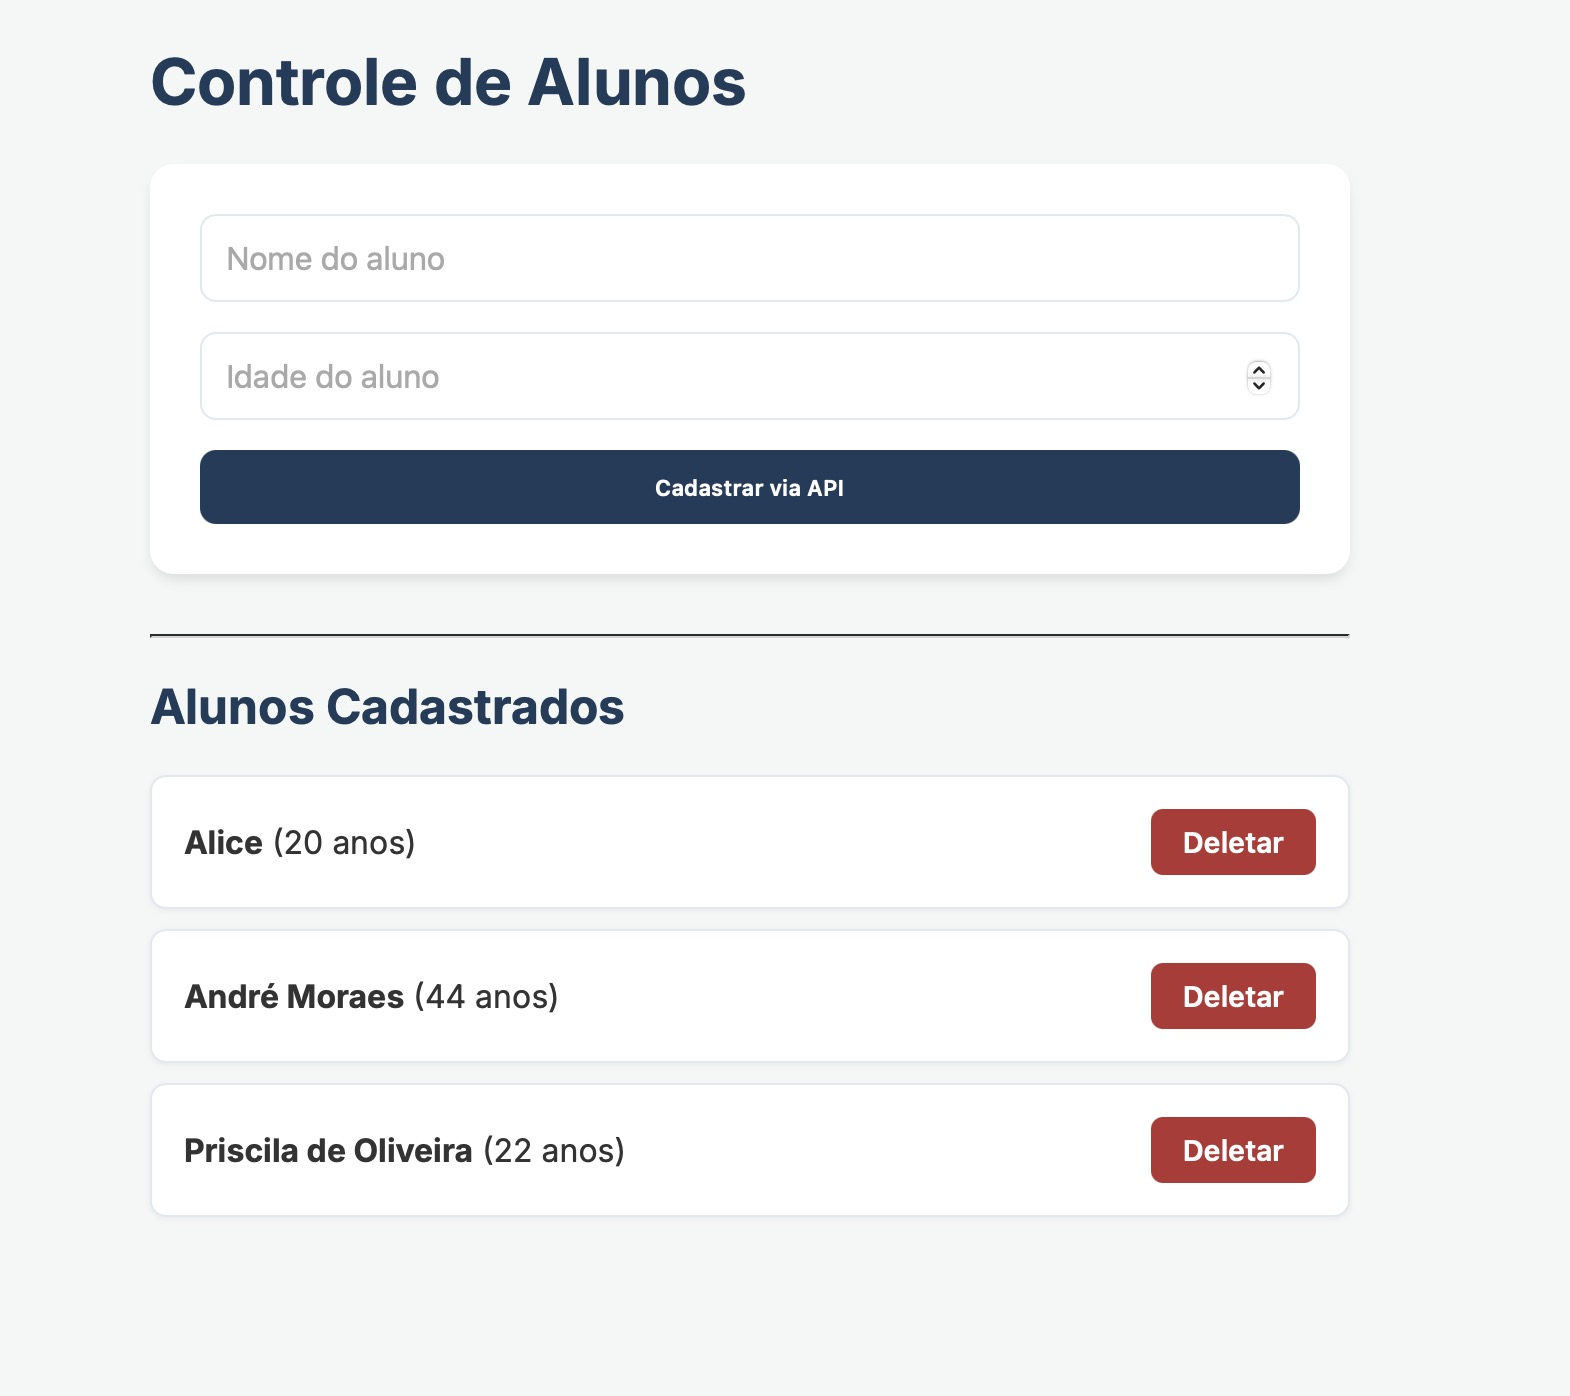
\includegraphics[width=0.88\textwidth]{roteiro-7-resultado.jpg}
\end{center}
\end{boxResultado}

\vspace{0.5cm}

A Figura abaixo mostra a aba \textbf{Rede (Network)} do DevTools com o filtro \textbf{Fetch/XHR} ativo, evidenciando as requisições assíncronas realizadas pela aplicação em segundo plano — sem recarregar a página:

\begin{boxResultado}[Requisições Assíncronas — Filtro Fetch/XHR no DevTools]
\begin{center}
    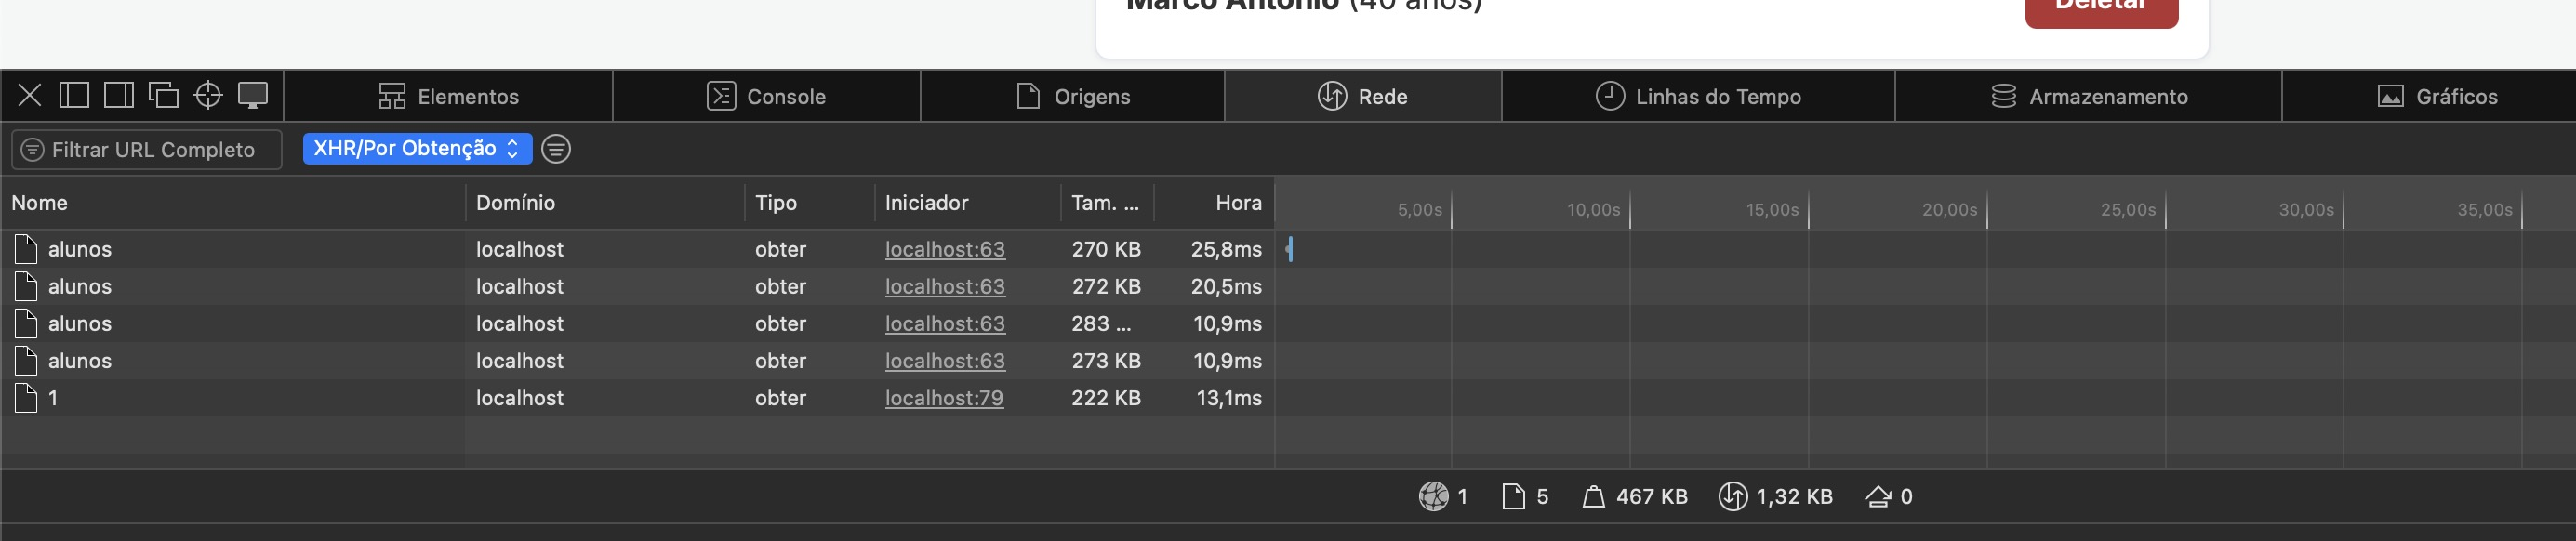
\includegraphics[width=0.88\textwidth]{roteiro-7-filtro-fetch-xhr-resutltado.jpg}
\end{center}
\end{boxResultado}


\subsection*{Estilização da Interface (Opcional — CSS Premium)}

Para dar um acabamento profissional e moderno à interface da sua aplicação Single Page Application (SPA), você pode criar uma folha de estilos personalizada.

Siga os passos abaixo para aplicar a estilização:
\begin{enumerate}
    \item Na raiz do seu projeto, crie uma pasta para arquivos estáticos e crie o arquivo CSS:
    \begin{boxCodigo}
    \begin{verbatim}
    mkdir static
    # Crie o arquivo static/style.css
    \end{verbatim}
    \end{boxCodigo}
    \item Adicione as seguintes regras CSS premium ao arquivo \texttt{static/style.css}:
    \begin{boxCodigo}
    \begin{verbatim}
    @import url(
      'https://fonts.googleapis.com/css2?family=Inter:wght@400;700'
    );

    :root {
        --bg-color: #f4f7f6;
        --card-bg: #ffffff;
        --primary-color: #1e3c5a;
        --primary-hover: #122538;
        --text-color: #333333;
        --border-color: #e2e8f0;
        --danger-color: #b43232;
        --danger-hover: #8c2525;
    }

    body {
        font-family: 'Inter', sans-serif;
        background-color: var(--bg-color);
        color: var(--text-color);
        max-width: 600px;
        margin: 40px auto;
        padding: 20px;
    }

    h1, h2 {
        color: var(--primary-color);
        font-weight: 700;
    }

    form {
        background-color: var(--card-bg);
        padding: 25px;
        border-radius: 12px;
        box-shadow: 0 4px 6px -1px rgba(0,0,0,0.1);
        margin-bottom: 30px;
        display: flex;
        flex-direction: column;
        gap: 15px;
    }

    input {
        padding: 12px;
        border: 1px solid var(--border-color);
        border-radius: 8px;
        font-size: 1em;
        outline: none;
        transition: border-color 0.2s, box-shadow 0.2s;
    }

    input:focus {
        border-color: var(--primary-color);
        box-shadow: 0 0 0 3px rgba(30,60,90,0.15);
    }

    button[type="submit"] {
        padding: 12px;
        background-color: var(--primary-color);
        color: white;
        font-weight: 600;
        border: none;
        border-radius: 8px;
        cursor: pointer;
        transition: background-color 0.2s, transform 0.1s;
    }

    button[type="submit"]:hover {
        background-color: var(--primary-hover);
    }

    button[type="submit"]:active {
        transform: scale(0.98);
    }

    ul {
        list-style: none;
        padding: 0;
        display: flex;
        flex-direction: column;
        gap: 10px;
    }

    li {
        background-color: var(--card-bg);
        padding: 16px;
        border-radius: 8px;
        box-shadow: 0 1px 3px rgba(0,0,0,0.05);
        display: flex;
        justify-content: space-between;
        align-items: center;
        border: 1px solid var(--border-color);
        transition: transform 0.2s;
    }

    li:hover {
        transform: translateY(-2px);
    }

    .btn-deletar {
        background-color: var(--danger-color);
        color: white;
        padding: 8px 16px;
        border: none;
        border-radius: 6px;
        font-size: 0.9em;
        font-weight: 600;
        cursor: pointer;
        transition: background-color 0.2s;
    }

    .btn-deletar:hover {
        background-color: var(--danger-hover);
    }
    \end{verbatim}
    \end{boxCodigo}
    \item No arquivo \texttt{templates/index.html}, adicione o link para o CSS dentro da tag \texttt{<head>}:
    \begin{boxCodigo}
    \begin{verbatim}
    <link rel="stylesheet" href="/static/style.css">
    \end{verbatim}
    \end{boxCodigo}
    \item Para que o botão de deletar adote o estilo correto, mude sua classe no script do \texttt{index.html}:
    \begin{boxCodigo}
    \begin{verbatim}
    <button class="btn-deletar" 
            onclick="deletarAluno(${aluno.id})">
        Deletar
    </button>
    \end{verbatim}
    \end{boxCodigo}
\end{enumerate}


\subsection*{Entrega}
O estudante deverá demonstrar ao professor:
\begin{itemize}
    \item A API respondendo a lista de alunos em formato JSON via endpoint GET;
    \item A inserção dinâmica de novos alunos sem recarregar a tela (POST);
    \item A remoção assíncrona do elemento HTML correspondente ao clicar em "Remover" (DELETE).
\end{itemize}

\end{document}
